\documentclass[prodmode,acmtecs]{acmsmall} \usepackage[ruled]{algorithm2e}
\usepackage{graphicx}

\acmYear{2015}
\acmMonth{4}

\begin{document}
\title{The Performance Characteristics of Astronomical Source Finders}
\author{YASEEN HAMDULAY
\affil {University of Cape Town}
}

\begin{abstract}
MeerKAT and ASKAP will run the biggest Hydrogen surveys ever completed. Our current source
finders will be unable to cope with such large surveys. We will look at different source
finding algorithms and techniques for accelerating them.
\end{abstract}

\keywords{Source Finding, Astronomy, GPU}

\acmformat{Yaseen Hamdulay, 2015. The Performance Characteristics of Astronomical Source Finders}

\maketitle

\section{Introduction}
Source finding within blind Hydrogen surveys is a computationally intensive but important process.
We are currently able to perform source finding on existing hydrogen surveys in less time than it takes
to record the data. However we do not expect our current source finding tools to be able to do this with
data coming from upcoming Radio Telescopes. 

The Australian Square Kilometre Array Pathfinder and MeerKAT is expected to begin observations in the latter
half of 2017. ASKAP is expected to produce approximately 80 terabytes of data per 8 hours of 
observation time. \cite{whiting2012source} ran a much smaller cube of 24GB of HIPASS \cite{wong2006northern}
 survey data on the Epic super-computing
cluster with 9600 cores and it took between a few minutes and a few hours depending on the
type of search. At this rate of processing ASKAP's expected workload will take days to months. 

Previous attempts at reducing execution time involved converting from single threaded code
to multi-threaded code across multiple CPU cores. \cite{scott} This gave really good results
but not enough to handle MeerKAT and ASKAP loads.

We are reaching the end of Moore's law for single cores. In order to continue improve overall performance
the number of concurrent threads are increasing to compensate for decreasing gains in single
threaded performance \cite{michalakes2008gpu}. GPU's are the embodiment of this philosophy
and can have hundreds of arithmetic cores. 

We have seen in \cite{fluke2011astrophysical}\cite{westerlund2015performance} that replacing CPU's with GPU's in Astronomy applications
can drastically decrease the execution time of astronomical calculations but more specifically
source finding algorithms.
\cite{holwerda2010trumpeting}
\cite{whiting2012source}
\cite{floer2014source}

\section{Comparison of Existing Source Finding Algorithms}
    Source finders operate on a data cube as input which consists of two spatial dimensions
    and one spectral dimension. Sources are sparse within the data cube with the rest
    dominated by noise. \cite{walsh2012maser}

    There are two important metrics used to describe source finding algorithms, completeness and 
    reliability. \cite{popping2012comparison}

    Completeness is defined as the ratio of sources found by the source finder
    in a given data cube to the number of actual sources within the data cube. This means that
    for a given source in a data cube a high completeness ratio means that the source finder is 
    very likely to detect this source and low completeness means that it could be overlooked.

    Reliability
    is the ratio of true positive source detections to the number of total detections. High reliability
    implies that a source finder will detect the majority of sources that exist within a data cube. 

    The flux density of a source is the sum of the intensities of all the detections or voxels 
    that contribute to the source. A source of low flux is generally much further away and harder
    to distinguish from noise.

    We want a source finder to have high reliability and high completeness.
    Since we care about accelerating these algorithms, their complexity and existing 
    acceleration attempts are important to consider.

    The Source Finder Accuracy Evaluator is a tool that takes a source finder as input and deterministically
    evaluates the source finders reliability and completeness characteristics. It does this
    by running the source finder over a known data cube that has a known catalogue of sources
    and comparing the output of the source finder with this known value. \cite{westerlund2012assessing}

    
    We will now compare these characteristics of different source finding algorithms.

 \cite{westerlund2012assessing}
 \cite{popping2012comparison}

    \subsection{2D-1D Wavelet Reconstruction}
    This source finding algorithm by Floer and Winkel functions by performing a transformation similar to a Fourier
    transformation called a wavelet transformation. This transformation finds coefficients $w_j(x)$
    so that we can decompose our original data $D(X)$ in the following way:

    $$D(x) = c_J(x) + \sum\limits_{j=1}^J w_j(x)$$
    
    We can find these coefficients efficiently with the ``algorithm \`{a} trous''. We
    use this decomposition to denoise by removing all $w_j(x)$ coefficients where
 $$w_j(x) < 5\text{ std. deviation}\{w_1, \ldots, w_n\}$$
    This works because the signal is sparse in the data. For most efficacy we can repeat this
    process a few times. We then reconstruct the signal and do intensity thresholding on the resultant
    data cube sans noise. 
    
    The completeness of this finder at low flux is close to 0\% 
    to almost 100\% completeness at high flux with almost as good performance as Duchamp. When using
    this source finder an alternative source finder should be used to detect sources at low flux. 
    Duchamp is superior in completeness and reliability to 2D-1D wavelet reconstruction across all flux values. \cite{popping2012comparison}
    
    It is noted that since the wavelet transformation of each spectral line is independent they
    can be computed in parallel. The memory use of this algorithm is $O(N_1 N_2 N_3 J_1 J_2)$ where $N_i$
    are the data cube dimensions and $J_i$ are the scales considered on each dimension. This is more
    memory than required by the other source finders which could make it slow or difficult on a memory
    constrained platform such as a GPU. 
    
    \cite{floer20122d}

     \subsection{CNHI}
     The Characterised Noise $H_1$ Source Finder is unique in function and has an innovative conceptual framework. Most other 
    source finders looked at the structure of the expected source and
     removed everything that did not look like a source with the assumption that it is noise.
     This limits the finder to sources whose structure we understand and goes against the 
     philosophy of a blind survey. 
     CNHI does the inverse of this. It characterises noise and removes everything that
     looks like noise. \cite{jurek2012characterised}
     
     This is an improvement over thresholding techniques that allegedly become more inaccurate
     as the resolution of radio telescopes increases. The inaccuracy is due to faint sources
     being spread out over more voxels decreasing average intensity but the noise floor will
     remain at the same level. 
     
     The CHNI algorithm works by applying the Kuiper test to a spectral line and find sections 
     that look different from the rest of the spectral line (using the assumption that the
     observation is dominated by noise). Overlapping sections are removed by choosing the 
     section with the largest Kuiper test value; the chosen section will have the lowest probability
     of being noise. The Kuiper test is then applied to these sections at multiple scales to
     find the galaxies within these sections. Objects immediately adjacent to each other
     are combined into a single object with the Lutz one-pass algorithm.
     
     Despite the innovative conceptual framework the performance of CHNI is poor across all
     flux levels in comparison to the other source finders. The output of CNHI has many 
     false positives and low completeness. \cite{popping2012comparison}
     
     \subsection{Duchamp}
Duchamp is primarily a thresholding source finder. Duchamp goes through four main phases during source finding.
Noise removal, searching, merging and parameterisation. During the noise removal step the user can either smooth the data
via convolution with a kernel or use wavelet construction in a manner very similar to 2D-1D wavelet
reconstruction discussed above. The searching is done by considering each channel as a plane and running the two dimensional
Lutz algorithm which scans each horizontal row and joins close objects \cite{lutz1980algorithm}. Once we have searched the entire
space we combine all objects that are within a user defined distance from each other. Every objects position
and flux values are calculated and added to the output catalogue. \cite{whiting2012duchamp}


The Duchamp source finding strategy  is the most reliable and complete of all strategies tested 
by Popping et al. This makes it an ideal candidate for acceleration as it could
be the most useful for use by large future hydrogen surveys. 

\subsection{Gamma Finder}
The Gamma finder is based on the Gamma Test. This finder smooths each spectral line with a Hanning
smoother. It then applies the Gamma test over a sliding window of constant width. The Gamma test will
find discontinuities or peaks over the spectral line, these discontinuities will correspond to sources. 
Due to the sliding window this finder struggles with broad sources that are larger
than the sliding window width as there are not any peaks in the center of a source. This is fixed by
running the Gamma test over the data with varying smoothing widths giving varying widths of each source.
\cite{boyce2003gammafinder}

According to \cite{popping2012comparison} the Gamma finder does not perform well with broad galaxies
despite the modification mentioned above. The completeness of the Gamma finder almost reaches that of Duchamp consistently over various flux values. 
This can be seen in figure 1 below. Unfortunately the reliability is not as good as its completeness. 
The realiability can be as low as 12\% for certain inputs. 

\begin{center}A table comparing the characteristics of various Source Finders \cite{popping2012comparison} \end{center}
    \begin{tabular}{|l | l | l | l | }
    \hline
    Name  & Completeness & Reliability & Parallelism \\
    \hline
    \hline
    Duchamp  & High & High & Multi-core CPU \\
    \hline
    CNHI  & Low & Low & Single thread \\
    \hline
    2D-1D wavelet reconstruction & High & High & Single thread \\
    \hline
    Parallel Gaussian  & Unknown & Unknown & GPU and CPU \\
    \hline
      Gamma Finder & Medium & Very low & Single thread \\
    \end{tabular}
    \\
\begin{figure}
  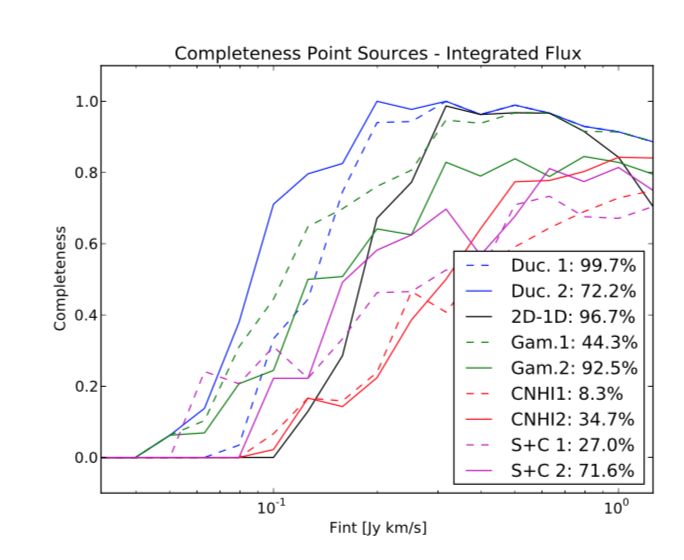
\includegraphics{comparisoncompleteness}
  \caption{Graph comparing the completeness of various Source Finders with reliability in the legend}
\end{figure}
\section{Source Finding Platforms}
    \subsection{Duchamp}
Duchamp is the most well-known source finding platform. It is written entirely in C++ and primarily uses
thresholding with various noise filtering schemes. The choice of noise filtering and thresholding
value is defined by the user at runtime.  
        \cite{whiting2012duchamp}

Duchamp in its current state runs on a single CPU core. There have been multiple attempts to run
parts of the Duchamp pipeline over multiple CPU cores \cite{scott} \cite{whiting2012source}. Badenhorst et al 
 successfully sped up the \`{a} trous noise suppression algorithm, which was the greatest contributor to the 
execution time, by 13x with eight threads on a quad-core CPU.
This speed up came with a 6x memory usage penalty. They found that with the speed up in the noise
suppression the execution time is now dominated by the statistics section of the pipeline. Finally,
they note that a CPU-GPU interaction has the potential to dramatically increase performance.

Selavy \cite{whiting2012source} is a distributed version of Duchamp that runs across multiple CPU
\cite{} cores across multiple hosts. It too accelerated the noise suppression algorithm. 
It was designed to run on a cluster of nodes each with 8 - 12
CPU cores where the entire data cube is unable to fit onto a single node. 


    \subsection{SoFiA}
    SoFiA is a modern flexible source finder framework that implements three different source finders
    and filters. SoFia is written in Python and C++ and is much newer than both Duchamp and SSoFF. 
    SoFiA's main advantage is its variety of source finders and filters.  
    SoFiA loads entire data cube into memory when performing source finding which will not scale to ASKAP
    and MeerKAT data sizes. Modifications need to be made in order to temporarily store parts of the data cube
    on disk.
    The filters implemented by SoFia are Convolution, 2D-1D wavelet reconstruction and noise normalisation.
    The source finders implemented by SoFia are the Threshold finder, Source and Clip and the Characterised Noise
    finder. 
        \cite{serra2015sofia}
        
     

        \subsection{SSoFF}
The Scalable Source Finding Framework  is designed to distribute source finders over High Performance
Computing clusters using the Message Passing Interface. It abstracts the concept of a source finder from
the task of parallelisation. The Parallel Gaussian Source Finder is implemented on top
of this framework in both the multi-core CPU and GPU variations.



\section{Acceleration Methods}
    \subsection{Multi-core CPU}
    Acceleration using multiple CPU cores is much easier than porting to GPU and happens more often as the techniques
    and technology has been around for longer. {\cite{fluke2011astrophysical}
    Writing multi-core CPU code can be as simple as adding a compiler directive for OpenMP\cite{cavuoti2014astrophysical}.

    The parallelism gained by multi-core CPU acceleration can be used to gauge the potiential speedups
    to be gained by implementing an algorithm on the GPU. If we cannot get a speedup by running
    on multiple CPU cores we are highly unlikely to get a speedup by porting to a GPU. 
    
        \cite{westerlund2014framework}
        \cite{scott}

    \subsection{GPU}
Graphics Processing Units are highly parallel processors that have a large amount of
arithmetic processing units when compared to CPU's which is dominated by control units
and cache memory. This is suited to computations done by astronomers with many reporting 
10 - 100x speed ups in their computations. \cite{hassan2011unleashing} 

An important metric to consider when doing source finding on MeerKAT data is recognising that
MeerKAT is in the desert with very little access to power. GPU's give the highest flops per watt
ratio making it a very useful tool for this problem.

However this does not come for free, coding on a GPU takes more time and is more complex than on a CPU. 

Due to the large amount of GPU arithmetic cores a brute force algorithm can often beat
a more complicated but clever solution.  \cite{fluke2011astrophysical} This implies that a direct port from
a CPU algorithm to a GPU is often not possible or will give bad results. It is necessary to think about the programs original
assumptions and see if they apply to the GPU. 

This is characterised by the APOD methodology for accelerating algorithms on GPU's: Assess, Parallelise, 
Optimise and Deploy \cite{cavuoti2014astrophysical}. The assess step tells us to identify portions of the
algorithm that would benefit from GPU acceleration. After identification we port the section of code
to the GPU. The optimise step involves running our accelerated code through a profiler to see whether 
there are more gains to be made in maximising throughput. The last step involves running the new
accelerated code and comparing it with the original serial algorithm. This is the process
that should be followed when accelerating the source finding algorithm. 

    \cite{laidler2013detection}
    

    \begin{tabular}{ |l|l|l| }
    \hline
    Name & Implementation time & Speedup \\
    \hline
      Single threaded CPU & Easy & 1x \\
    \hline
    Mult-threaded CPU & Easy & 1x - 5x  \\
    \hline
    GPU & Difficult & 2x - 100x  \\
      \hline
    \end{tabular}
    \\
\begin{center}    Comparison of acceleration methods\end{center}

\section{Existing Accelerated Source Finders}
The filtering portion of the Parallel Gaussian Source finder \cite{westerlund2015performance}
has been ported to run on a GPU. It originally took up 70\% of the execution time.
This filter has been sped up by 3.6x and the source finder has been sped up by 2x overall. 
There are a few optimisations that can be done to improve the performance of the GPU accelerated
source finder that has not been done by this study. 

5 - 10\% of execution time is spent copying data from the Host onto the GPU. This can be reduced by streaming
data into the GPU and have it process the data as it arrives instead of waiting for the entire
data cube to be copied. Another large contributor is the statistics functions. This was not such
a large contributor before the filter was parallelised but now dominates the execution time,
this is the next candidate for parallelisation. 

As the data cube is split over more nodes we get diminishing returns of performance increases.
This occurs because more and more of the data per node is dominated by ``halo data''.

\section{Discussion}
CNHI had an interesting conceptual framework 
but did not perform as well as expected despite the theoretical problems it solved. 2D-1D wavelet
reconstruction performed almost as well as Duchamp. This is likely due to Duchamp using wavelet deconstruction
as one of its noise removal procedures. The Gamma finder has really high completeness but disappointingly
low reliability. This is not a very good result. A source finder that reports all points on the cube as sources will
have 100\% completeness and 0\% reliability which is almost as bad as the performance of Gamma finder.

Duchamp is a clear winner out of the source finders tested.    
It has also been proven to parallelise well by the CPU parallelism attempts. This will hopefully 
make GPU parallelism easier. 

\section{Conclusions}
We have seen that porting serial code to a Graphics Processing Unit can give multiple order of magnitude speedups in
execution time. Porting a source finder would move us closer to our goal of performing source finding
on future ASKAP and MeerKAT data. 

We have seen an example of this by the GPU version of the Parallel
Gaussian Source Filter.

Despite there already existing an accelerated GPU source finder it is still necessary to port 
more source finders as each have very different completeness and reliability characteristics. 

After analysing the various source finders we conclude that Duchamp is the best candidate for 
GPU acceleration due to its completeness, reliability and its maturity.
 
\bibliographystyle{ACM-Reference-Format-Journals}
\bibliography{litreview}

\end{document}
